% !TEX root = main.tex

This section presents and discusses the experimental results obtained by the
four classifiers on domain~1 (digits) and domain~4 (3D figures), under both
the user-independent and the user-dependent cross-validation protocols.
We first report the best hyperparameter configurations selected on the
inner-validation folds, then the test accuracies, the statistical comparison
of the methods, and finally a per-class confusion analysis of the best model.

% ----------------------------------------------------------------
\subsection{Best hyperparameter configurations}
\label{subsec:best_config}
% ----------------------------------------------------------------

For every (method, domain, CV-mode) combination, the configuration achieving
the highest mean inner-validation accuracy was retained and re-fitted on the
full outer training fold. The resulting selections are reported in
Table~\ref{tab:best_config}. They are remarkably stable across the four
experimental settings, which suggests that the chosen grids cover sensible
operating points and that the selected configurations do not overfit the
inner-validation set.

\begin{table}[H]
\centering
\caption{Best hyperparameter configurations selected by inner-validation,
per method, domain and CV protocol. ``--'' means the hyperparameter does not
apply.}
\label{tab:best_config}
\resizebox{\linewidth}{!}{%
\begin{tabular}{l l c c c c}
\toprule
\textbf{Method} & \textbf{Hyperparameter}
  & \multicolumn{2}{c}{\textbf{Domain 1 (digits)}}
  & \multicolumn{2}{c}{\textbf{Domain 4 (3D figures)}} \\
\cmidrule(lr){3-4}\cmidrule(lr){5-6}
 & & user-indep. & user-dep. & user-indep. & user-dep. \\
\midrule
\multirow{2}{*}{DTW}
  & PCA                   & none & none & none & none \\
  & $k$-NN neighbours $k$ & 1    & 1    & 1    & 1    \\
\midrule
\multirow{4}{*}{Edit-distance}
  & PCA                   & none & none & none & none \\
  & Codebook size $K$     & 40   & 35   & 20   & 40   \\
  & Compression           & No   & No   & No   & No   \\
  & $k$-NN neighbours $k$ & 1    & 1    & 1    & 1    \\
\midrule
\multirow{2}{*}{Three-Cents}
  & PCA                          & \textbf{2D} & \textbf{2D} & none & none \\
  & Resampling points $n$        & 16          & 16          & 16   & 16   \\
\midrule
\multirow{2}{*}{BiLSTM}
  & Sequence length $T$ & 64 & 16 & 16 & 64 \\
  & Hidden units $h$    & 64 & 64 & 32 & 64 \\
\bottomrule
\end{tabular}
}
\end{table}

Several observations can be drawn from Table~\ref{tab:best_config}. For the
two dynamic-programming baselines, the optimal $k$-NN neighbourhood size is
always $k = 1$: the closest single template is more discriminative than a
larger neighbourhood, indicating that the inter-class distances are large
relative to intra-class variability once a proper sequence metric is used.
Reducing the dimensionality of the trajectories with PCA never improves the
DTW or Edit-distance accuracies, which is expected since both methods already
exploit the full 3D geometry of the signal. For the Edit-distance baseline,
the selected codebook sizes ($K \in \{20, 35, 40\}$) cluster around the middle
of the grid; smaller values would produce overly coarse strings, while larger
values fragment the same trajectory shape into too many symbols and inflate
the edit cost. Disabling the compression of consecutive duplicate symbols was
systematically preferred: compression discards local timing information,
which apparently still carries discriminative signal even after vector
quantization.

The Three-Cents recognizer consistently selects $n = 16$ resampling points,
which is markedly lower than the $n = 64$ value used in the original \$1
recognizer~\cite{Wobbrock2007}. This is consistent with the short and
relatively simple trajectories of the considered domains: too dense a
resampling adds noise without bringing new geometric information. Interestingly,
the recognizer benefits from a 2D PCA projection on domain~1 (planar digits)
but prefers the full 3D coordinates on domain~4 (geometric figures, which are
intrinsically three-dimensional). This is precisely the behaviour one would
expect from a method that relies on a fixed point-to-point correspondence:
when the signal is intrinsically planar, removing the noisy out-of-plane
component sharpens the comparison.

Finally, the BiLSTM selects the smallest hidden state ($h = 32$) in the
hardest setting (domain~4, user-independent) and the largest ($h = 64$)
elsewhere, which is consistent with the well-known trade-off between model
capacity and overfitting on a $\sim$1\,000-sample dataset. The selected
sequence length $T$ varies between 16 and 64 frames without a clear pattern,
suggesting that the model is relatively robust to this choice.

\subsection{Classification accuracy}
\label{subsec:accuracy}

 
Table~\ref{tab:accuracy} reports the mean test accuracy and standard deviation
across the 10 cross-validation folds for each method, domain and CV protocol,
using the best configuration identified in Section~\ref{subsec:best_config}.
 
\begin{table}[H]
\centering
\caption{Mean test accuracy (\%) $\pm$ standard deviation across 10 folds.
Best result per column in \textbf{bold}.}
\label{tab:accuracy}
\resizebox{\linewidth}{!}{%
\setlength{\tabcolsep}{4pt}
\begin{tabular}{l cc cc}
\toprule
 & \multicolumn{2}{c}{\textbf{Domain 1}} & \multicolumn{2}{c}{\textbf{Domain 4}} \\
\cmidrule(lr){2-3}\cmidrule(lr){4-5}
\textbf{Method} & indep. & dep. & indep. & dep. \\
\midrule
DTW
  & $82.6 \pm 12.4$
  & $99.6 \pm 0.5$
  & $74.4 \pm 11.2$
  & $99.5 \pm 1.0$ \\
Edit-distance
  & $67.9 \pm 23.1$
  & $99.1 \pm 0.7$
  & $60.2 \pm 19.5$
  & $98.3 \pm 1.4$ \\
Three-Cents
  & $\mathbf{96.3 \pm 4.6}$
  & $\mathbf{99.8 \pm 0.4}$
  & $\mathbf{95.1 \pm 5.3}$
  & $\mathbf{98.6 \pm 1.3}$ \\
BiLSTM
  & $85.0 \pm 12.7$
  & $97.2 \pm 2.2$
  & $70.1 \pm 8.2$
  & $88.5 \pm 3.2$ \\
\bottomrule
\end{tabular}
}
\end{table}
 
Three main patterns emerge from Table~\ref{tab:accuracy}.
 
\textbf{User-dependent accuracy is systematically higher than
user-independent accuracy} for every method and every domain, confirming the
expected answer to~(Q2). The gain is particularly dramatic for the two
dynamic-programming baselines: DTW improves by $+17.0$ and $+25.1$ percentage
points on domains~1 and~4 respectively, while Edit-distance improves by $+31.2$
and $+38.1$ points. When the model has access to several repetitions of the
same gesture by the same user, the 1-NN rule becomes a near-trivial matching
task, which explains the near-perfect user-dependent scores
($\geq 98\%$) of DTW, Edit-distance and Three-Cents. The residual
gap observed for BiLSTM ($+12.2$ and $+18.4$ points) is comparatively small,
confirming that the main limitation of the neural approach is not the
user-shift per se, but the insufficient training-set size.
 
\textbf{Three-Cents is the best method in the user-independent setting} on
both domains, achieving $96.3\%$ on domain~1 and $95.1\%$ on domain~4 with a
low standard deviation ($\leq 5.3\%$), pointing to~(Q1). This result is
remarkable given the simplicity of the method: by omitting the rotation step
of the original \$1 recognizer and relying on a lightweight resample–scale–translate
pipeline, Three-Cents outperforms all competitors by a wide margin.
The runner-up is BiLSTM on domain~1 ($85.0\%$) and DTW on domain~4
($74.4\%$), both well below Three-Cents.
 
\textbf{Edit-distance is the weakest method in the user-independent setting}
and exhibits the largest variability (std up to $23.1\%$). The vector
quantization step, necessary to convert continuous 3D trajectories into
discrete symbol strings, entails a lossy compression of the geometric
information. When templates come from different users (user-independent case),
this loss is compounded by inter-user style variability, leading to
inconsistent codebook assignments and poor generalization. In the
user-dependent setting, however, Edit-distance nearly saturates ($\geq 98\%$),
showing that the method is not fundamentally flawed but simply sensitive to
the covariate shift introduced by unseen users.

\subsection{Statistical comparison of the methods}
\label{subsec:stats}

 
Statistical tests were conducted on the user-independent setting, which is
the most practically relevant scenario and the one addressed by research
question~(Q3). Following the recommendation of Dem\v{s}ar~\cite{Demsar2006}
for comparing multiple classifiers across several datasets, we first applied
the non-parametric \textbf{Friedman test} to assess whether at least one
method differs significantly from the others (null hypothesis: all methods
share the same expected rank). The test was highly significant in both domains
($\chi^2 = 23.03$, $p < 0.001$ for domain~1; $\chi^2 = 24.15$, $p < 0.001$
for domain~4), firmly rejecting the null hypothesis and justifying post-hoc
pairwise comparisons.
 
Post-hoc analysis was carried out with two complementary procedures.
The \textbf{Nemenyi test} computes a critical difference
$\mathrm{CD} = 1.48$ (at $\alpha = 0.05$, $k = 4$ methods, $N = 10$ folds):
two methods are declared significantly different if and only if their average
Friedman ranks differ by more than CD. Results are visualised in
Figure~\ref{fig:cd_diagrams}, where methods connected by a horizontal bar are
\emph{not} significantly different. The \textbf{Wilcoxon signed-rank test}
with Holm--Bonferroni correction was additionally applied to each pair,
providing fold-level evidence that is more sensitive than the rank-based
Nemenyi test.
 
\begin{figure}[!h]
  \centering
  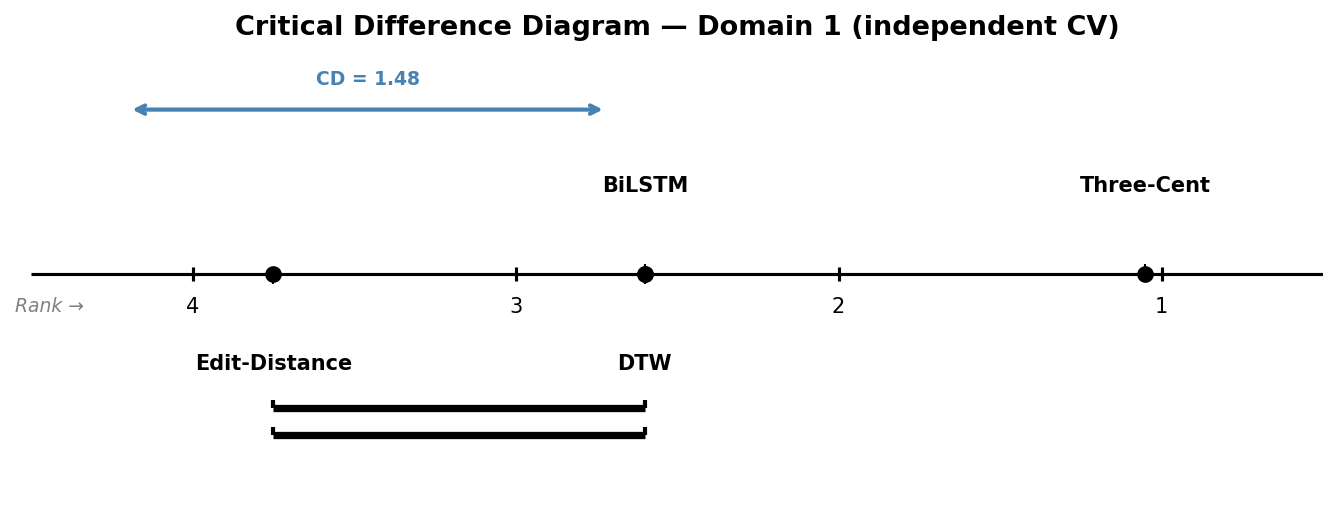
\includegraphics[width=\linewidth]{figures/cd_diagram_domain1_independent.png}
  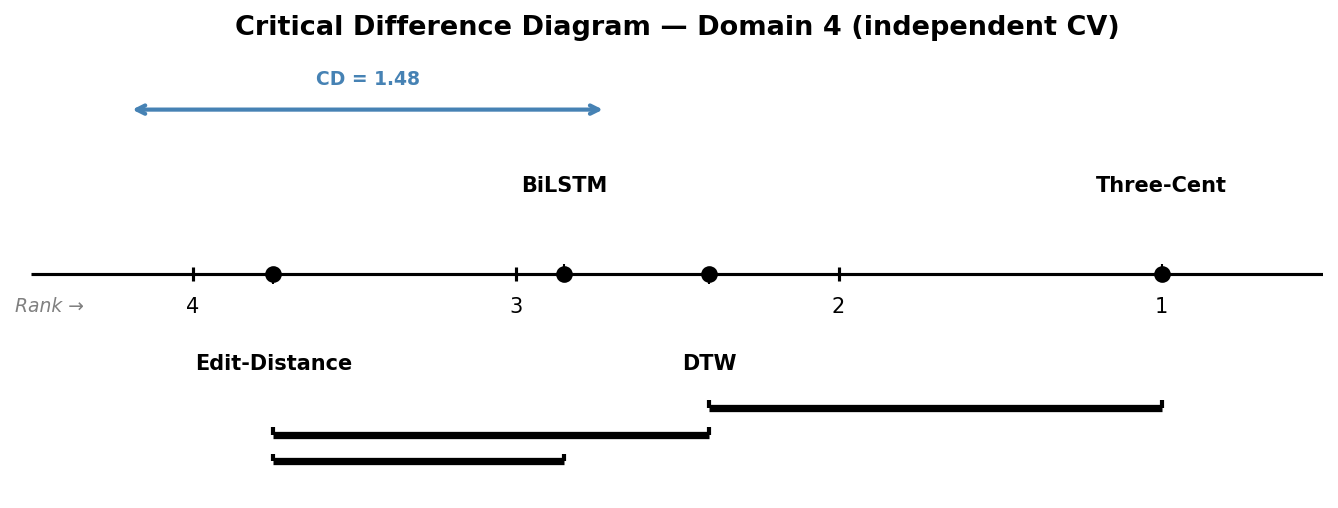
\includegraphics[width=\linewidth]{figures/cd_diagram_domain4_independent.png}
  \caption{Critical difference diagrams (Nemenyi, $\alpha = 0.05$) for
  domain~1 (top) and domain~4 (bottom) under user-independent CV\@.
  Methods are ranked from best (right, rank~1) to worst (left, rank~4).
  Horizontal bars connect methods whose rank difference does not exceed
  $\mathrm{CD} = 1.48$, i.e.\ whose performance is \emph{not} statistically
  distinguishable.}
  \label{fig:cd_diagrams}
\end{figure}
 
The diagrams lead to the following conclusions regarding~(Q3).
 
On \textbf{domain~1}, Three-Cents (avg.\ rank~1.05) stands isolated on the
right, connected to no other method: it is significantly better than DTW
(Wilcoxon adj-$p = 0.016$), Edit-distance (adj-$p = 0.012$) and BiLSTM
(adj-$p = 0.010$). DTW and BiLSTM share the same average rank (2.60) and are
not distinguishable from each other (adj-$p = 0.625$). The Wilcoxon--Holm
procedure does however separate Edit-distance from both DTW (adj-$p = 0.031$)
and BiLSTM (adj-$p = 0.023$), a difference the less powerful Nemenyi test
cannot detect.
 
On \textbf{domain~4}, Three-Cents (avg.\ rank~1.00) is again the sole
top-ranked method, significantly outperforming Edit-distance
(adj-$p = 0.010$), DTW (adj-$p = 0.012$) and BiLSTM (adj-$p = 0.008$). The
three remaining methods form a partially indistinct group: Edit-distance and
BiLSTM are not separable under either test, and DTW versus BiLSTM is also
non-significant (adj-$p = 0.238$). DTW does however significantly outperform
Edit-distance under Wilcoxon--Holm (adj-$p = 0.012$).
 
In summary, \textbf{Three-Cents is the only method that is statistically
superior to all others in both domains} under the user-independent protocol,
providing a clear and unambiguous answer to~(Q3). No other pairwise ordering
is consistently significant across both domains.